\documentclass[a4paper]{article}
\usepackage{cmap}
\usepackage{url}
\usepackage[utf8]{inputenc}
\usepackage[russian]{babel}
\usepackage{graphicx}
\graphicspath{{img/}}
\addto{\captionsrussian}{\renewcommand{\refname}{References}}
\addto{\captionsrussian}{\renewcommand{\abstractname}{Abstract}}
\addto{\captionsrussian}{\renewcommand{\figurename}{Fig.}}
% \frenchspacing
\begin{document}
\author{Victor Bocharov\\\small Mathlingvo\\\small\tt bocharov@opencorpora.org\and Svetlana Bichineva\\\small St.\,Petersburg State University\\\small\tt\ bichineva@opencorpora.org\and Dmitry Granovsky\\\small Mathlingvo\\\small\tt grand@opencorpora.org\and Natalia Ostapuk\\\small St.\,Petersburg State University\\\small\tt\ nataxan90@gmail.com\and Maria Stepanova\\\small St.\,Petersburg State University\\\small\tt\ mariarusia@gmail.com}
\title{Quality Assurance Tools in the OpenCorpora Project}
\date{}
\maketitle
\begin{abstract}
OpenCorpora is a project that aims at creating an annotated corpus of Russian texts, which will be fully accessible to researchers, the annotation being crowd-sourced. The article deals with annotation quality assurance tools.
\end{abstract}
\section{Introduction}
One would think that finding a corpus of Russian texts, including annotated one, could not be a problem at the moment. Moreover, some of the corpora are accessible on the Internet (see survey in~\cite{reznikova05}), which we think considerably increases their value for the linguistic community. To the best of our judgment, accessibility on the Internet usually means that there is an interface that may be used to submit parameterized search queries to the corpus. Of course, this makes possible various theoretical linguistic research, which requires analysis of word usage, frequency etc. However, this is not sufficient for the corpus to be used as a resource for machine learning or testing applications such as morphological parsers or disambiguation systems, because in these cases we need the annotated texts themselves rather than the search results. In principle it is possible to obtain the annotation from the existing corpora, but one faces a lot of trouble of either technical, administrative or proprietary kind.

This state of affairs motivated the OpenCorpora project, intending to create an annotated corpus of Russian texts. The content of the corpus will be accessible to everyone under a free license, the annotation being crowd-sourced. This has so far proved to be a good editing model in a number of projects, the best known of them, perhaps, Wikipedia~\cite{enwiki}. It has been recently demonstrated that crowd-sourcing is a suitable method for obtaining linguistic data and ``the quality is comparable to controlled laboratory experiments, and in some cases superior''~\cite{munro10} (another survey on crowd-sourcing in linguistics is provided in~\cite{wang10}). In OpenCorpora project we are working on crowd-sourcing linguistic annotation. In the near future the primary issue is the morphological annotation, the syntactic and semantic ones are to follow. Our goal is to collect high-quality manual annotation which will then be used to train disambiguation tools and other kinds of software.

OpenCorpora will include texts obtained from sources where copying and redistribution is legally allowed, i.e. texts with CC-BY-SA compatible license or public domain texts. CC-BY-SA compatible sources are: Wikimedia projects (Wikipedia and WikiNews~\cite{enwikinews}), www.chaskor.ru news agency. Many texts of Russian classic literature are in public domain and are available from WikiSource~\cite{enwikisource}.

Crowdsourcing being the main method of aggregating materials, it is essential to make the quality of the results a priority since it is impossible to know users' qualification in advance. Moreover, quality assurance should be as automated as possible. Drawing experts into the annotation verification is unacceptable (due to the high cost of human labor) although it may be necessary in certain cases. The main QA tools of the morphological annotation are a model of grammatical labels compatibility and morphological dictionary. Both instruments are used to describe acceptable combinations of grammatical labels. Whenever an unacceptable input combination occurs, the software produces an error message. In OpenCorpora we use warnings as error reports, which do not block user's activity. The aim of such warnings is to draw user's attention to the potentially erroneous input. It is the user who has the final say.

The article will further deal with the OpenCorpora project itself, its morphological dictionary structure and compatibility models for grammatical labels.
\section{About the OpenCorpora project}
OpenCorpora includes a linguistically annotated corpus of Russian texts freely distributable under CC-BY-SA~\cite{cc-by-sa} licence and software to annotate it.

Under linguistic annotation we understand the following:
\begin{itemize}
\item segmentation of a character sequence into word forms, sentences and paragraphs;
\item morphology: specifying the part of speech and grammatical features of word forms, morphological disambiguation;
\item local syntax:
\begin{itemize}
\item specifying the borders of multiword entities (analytical verbal structures, compound comparatives and superlatives, compound numerals, compound conjunctions, prepositions and particles, adverbial, predicative and parenthetical clauses, names of people and objects, dates) and their grammatical features;
\item combining word forms into syntactic groups (nominal, prepositional, verbal, adjectival groups) and marking dependencies within groups;
\end{itemize}
\item lexical semantics: specifying a particular word sense for a word form.
\end{itemize}

Division into paragraphs is taken from the source and is intended mainly to facilitate adding new texts, though it well may be useful for a researcher, too. Division of a paragraph into sentences is done automatically and checked by users.

A sentence is divided into tokens also automatically with a manual check to follow. As a token we regard a minimal meaningful symbol sequence without spaces. Any token may be either a word form (that is present in the dictionary) or not. The latter case applies to e.g. punctuation marks, web addresses, formulae (chemical, mathematical etc.) and other character combinations not kept in the dictionary, for example, due to their infinite number.

The unit of morphological annotation is a token. The annotation of a token consists of one or several (in the case of homonymy) interpretations. Each interpretation must include the token class (present in the dictionary or not). For dictionary tokens it also includes:
\begin{itemize}
\item lemma ID from the dictionary;
\item part of speech;
\item a set of values of the obligatory grammatical categories (e.g. number for nouns);
\item a set of labels marking the features of the particular word form used in the text (e.g. ``misprint'', ``verb used impersonally'').
\end{itemize}

\begin{figure}[h!]
\center{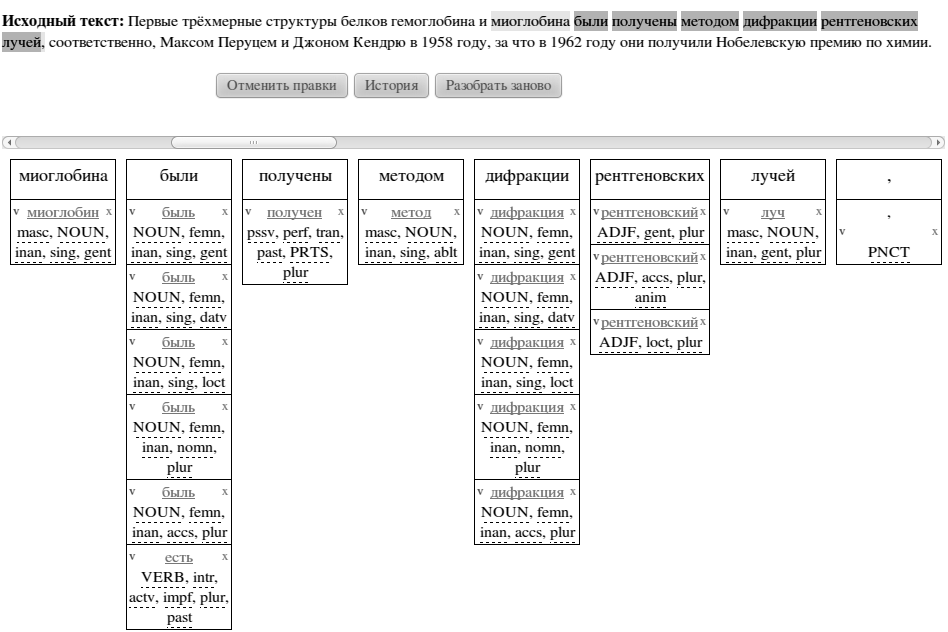
\includegraphics[width=1\linewidth]{2011_Dialog_img1.png}}
\caption{Morphological markup editor web-based user interface}
\end{figure}

Figure 1 shows a sentence morphological annotation fragment in annotation editor interface. The whole sentence is in the upper part. The part annotation of which fits the width of the edit window is highlighted. The annotation itself is represented in columns. Each column includes all the versions of morphological analysis of a word form. The word underlined is a hyperlink to the morphological dictionary. The ``v'' button in the left upper part is used to mark an option as the correct one and all the others as incorrect. The ``x'' button marks the selected option as incorrect.

The same information is available in the XML format. For the word form ``были'' it is as follows:
\begin{verbatim}
<tfr t="были">
  <v>
    <l id="4342" t="быль">
      <g v="NOUN"/> <g v="femn"/> <g v="inan"/> <g v="sing"/> <g v="gent"/>
    </l>
  </v>
  <v>
    <l id="4342" t="быль">
      <g v="NOUN"/> <g v="femn"/> <g v="inan"/> <g v="sing"/> <g v="datv"/>
    </l>
  </v>
  <v>
    <l id="4342" t="быль">
      <g v="NOUN"/> <g v="femn"/> <g v="inan"/> <g v="sing"/> <g v="loct"/>
    </l>
  </v>
  <v>
    <l id="4342" t="быль">
      <g v="NOUN"/> <g v="femn"/> <g v="inan"/> <g v="nomn"/> <g v="plur"/>
    </l>
  </v>
  <v>
    <l id="4342" t="быль">
      <g v="NOUN"/> <g v="femn"/> <g v="inan"/> <g v="accs"/> <g v="plur"/>
    </l>
  </v>
  <v>
    <l id="52243" t="есть">
      <g v="VERB"/> <g v="intr"/> <g v="actv"/> <g v="impf"/> <g v="plur"/>
      <g v="past"/>
    </l>
  </v>
</tfr>
\end{verbatim}
The software being developed within the OpenCorpora project is designed as a set of web applications, i.e. it is run on a web server and provides access to its functions via a web browser. The OpenCorpora web server implements the following functions:
\begin{itemize}
\item storing annotated texts and their edit history;
\item storing the dictionary and its edit history;
\item a web interface for annotation and dictionary editing;
\item quality assurance software.
\end{itemize}

The project is currently at the stage of developing the software for graphematic and morphological levels of annotation. The current version is available at \url{http://opencorpora.org}. At the moment the data on the website is for demonstrating the software functionality and for debugging.
\section{Morphological dictionary}
OpenCorpora uses AOT's~\cite{aot} morphological dictionary, customized for annotation quality assurance tasks. The dictionary is closely integrated with the corpus itself by numerical descriptors of lemmata~--- the components of word forms morphological interpretation in the annotations. This integration of text morphological annotation with the dictionary enables to solve the following problems:
\begin{itemize}
\item misprint checking at the stage of adding text to the corpus: trying to add a text with word forms not found in the dictionary will result in a warning;
\item morphological features acceptability checking: specifying in annotation a combination of grammatical labels, not stated in the description of the said lemma in the dictionary will result in a warning as well;
\item possibility to change lemma interpretation throughout the whole corpus: if lemma description in the dictionary is changed, all its entries in the corpus will be marked as requiring revision;
\item possibility to add lexical semantic information without changing annotation structure: one can divide certain lemmata into several units at the dictionary level thus stating that these units reflect different meanings of the lemma. The user who edits annotation can choose one of the lemma meanings for each its occurence in the corpus.
\end{itemize}

The unit of the morphological dictionary is a lemma. A lemma has the following properties:
\begin{itemize}
\item part of speech;
\item values of grammatical categories obligatory for the lemma of the given part of speech;
\item optional labels;
\item list of word forms;
\item list of links with other lemmata.
\end{itemize}

The following properties are specified for word forms:
\begin{itemize}
\item textual representation of the word form;
\item values of grammatical categories obligatory for the word form of the given part of speech;
\item optional labels.
\end{itemize}

The list of all possible grammatical labels is closed. Grammatical labels compatibility restrictions are described in the framework of compatibility model not designed to be changed frequently.
\section{Adaptation of AOT morphological dictionary}
Since the task of annotation correctness assurance is solved by means of the morphological dictionary, we needed to bring the dictionary to a form in which the correctness of dictionary data could be also verified automatically. The main changes followed two directions: paradigm grids unification and reduction of homonymic lemmata during automated morphological parsing. Besides that, we added to the dictionary a possibility to establish links between lemmata. Despite the fact that the format of dictionary representation has changed significantly, all the data presented in AOT was included to the OpenCorpora dictionary in one form or another to retain the possibility to review any decision without relaunching the procedure of dictionary transformation.

Paradigm grids unification means that lemmata of each part of speech have a set of acceptable forms and grammatical features. Acceptable grammatical features are described within the model of grammatical categories compatibility, the list of acceptable forms being generated on its basis. Some lemmata in the AOT dictionary contain descriptions of forms of several parts of speech\footnote{Here we use term ``part of speech'' the same way it is used in AOT project (see \url{http://www.aot.ru/docs/rusmorph.html})} at the same time, e.g. verbs (infinitive, finite verb form, participles and gerund) and adjectives (the full and the short forms). Such lemmata were divided into several separate lemmata with links between them, the latter enabling us to restore if needed the fact that in the source dictionary it was one lemma.

Some parts of speech from the AOT dictionary were merged since they had the same sets of word forms and grammatical categories. Thus ordinal numerals and pronominal adjectives were joined to full adjectives as classes. Pronominal adverbs were added as a class of adverbs.

Reduction of homonymic lemmata during automated dictionary-based morphological text parsing was done to simplify morphological disambiguation. We tried either to eliminate the ambiguity at all whenever it was possible without information loss or to pass from lemma ambiguity to word form ambiguity within one lemma.

For instance, the word ``микроб'' may be either animate or inanimate. In the AOT dictionary such cases are described by means of two lemmata, which differ only in the form of accusative case. While transforming the dictionary, we merged such lemmata adding two alternative forms of accusative case.

Another example is the full adjectives, whose forms coincide with forms of full participles. We also united such lemmata, adding to the participles a label, stating that this lemma may be used as an adjective. In the course of morphological disambiguation in the text the user should retain or remove this label instead of choosing either full adjective or full participle. Since distinguishing between adjective and participle needs better qualification in the field of Russian grammar than distinguishing gender, case and number, such description form is more preferable, because anyone who is not enough sure about the first question can put the correct values of gender, case and number leaving the choice between adjective and participle to someone more competent. If adjectives and participles were different lemmata, the choice between them would have to be made before the choice of gender, case and number.

At the moment the possibility to establish links between lemmata is used only for joining the lemmata that have been divided into several parts, but it also can be used to describe other phenomena, e.g. different kinds of derivational relations, whenever we need them.

The changes described above are in fact technical changes of format without changing of content.
\section{Compatibility model for grammatical labels}
The compatibility model describes a set of possible grammatical labels, their applicability to the description of different objects and their co-occurrence possibility. Possible objects of description are the word forms in the annotation, lemmata and forms in the dictionary. Some grammatical labels can describe any of possible objects, e.g. the labels masc/femn/neut (masculine, feminine, neuter) are applicable to word forms, the lemmata of nouns and forms of adjectives. Uimp (impersonal use of a personal verb) is an example of a label applicable only to the word forms (i.e. only to the text annotation in the corpus rather than description of lemmata and forms in the dictionary).

Among grammatical labels in use we specify the following types:
\begin{itemize}
\item labels standing for the parts of speech (NOUN~--- noun, ADJF~--- full adjective, VERB~--- finite verb form, \ldots);
\item labels standing for the grammatical categories (CAse~--- case, NMbr~--- number, GNdr~--- gender, \ldots);
\item labels standing for the values of grammatical categories (sing~--- singular, nomn~--- nominative, 1per~--- first person);
\item labels marking a group of lemmata within one part of speech (Qual~--- qualitative adjective, Sgtm~--- singularia tantum, Geox~--- label for toponyms, \ldots);
\item labels referring to word form features but not being the values of some grammatical category (Erro~--- misprint, Infr~--- colloquial form).
\end{itemize}

The full current list of grammatical labels is available at \url{http://opencorpora.org/dict.php?act=gram}.

Relations determining the compatibility of grammatical labels and their applicability to certain objects are defined on the set of grammatical labels. It features the following types of relations:
\begin{itemize}
\item relation ``grammatical category~--- attribute'' (POST (part of speech)~--- NOUN, CAse~--- nomn, \ldots). The label which is the first element in the relation is a grammatical category. The second element in the relation is a value of this category.
\item relation of obligatory application for lemmata (NOUN~--- GNdr, PRTF~--- TEns). This relation describes a set of classifying categories for lemmata of the given part of speech. Lemmata of a noun must have a gender, lemmata of a full participle must have a tense (full participle is a separate lemma for reasons stated above).
\item relation of obligatory application for forms (NOUN~--- CAse, ADJF~--- GNdr). This relation describes inflectional categories. Nouns decline and adjectives change according to genders.
\item relation of optional application for lemmata (NOUN~--- Pltm, VERB~--- Impr). The relation describes possible but not obligatory labels. Some nouns were assigned the label Pltm (pluralia tantum), some verbs were assigned the label Impr (impersonal).
\item relation of optional application for forms (NOUN~--- nomn, VERB~--- 1per). This relation describes a possibility to apply a label to a word form of a given part of speech. Usually the relation is not defined manually but is determined automatically.
\item relation of incompatibility (plur~--- masc). The relation implies that both labels can not be applied to the word form at the same time. The values of the same category are incompatible, for example, plur and sing are incompatible for they are both the values of the category NMbr.
\end{itemize}

A set of relations of optional application is automatically deduced from the relations of obligatory applicability: if a grammatical category is obligatory for a form or a lemma, all its values are applicable for the form or the lemma. For example, the relations of optional applicability for a form NOUN~--- sing and NOUN~--- plur are automatically deduced from the relation of obligatory applicability for a form NOUN~--- NMbr.

Relations between grammatical labels are described as a table which is an integral part of the dictionary. The full current version of this table is available at \url{http://opencorpora.org/dict.php?act=gram_restr}.

The compatibility model is used to validate the dictionary and the morphological annotation in the following way:
\begin{itemize}
\item grammatical labels must be applicable to the objects they describe. If there is no explicit relation of applicability (either added manually or inferred on the basis of other relations) then the grammatical label is not applicable;
\item grammatical labels must be compatible, i.e. any labels explicitly marked as incompatible must not occur together with the same object.
\end{itemize}

The dictionary and annotation are validated automatically as the source data changes. The errors are entered in the table, which is available at \url{http://www.opencorpora.org/dict.php?act=errata}. These errors may be (or may be not) a reason for changing the dictionary or the annotation. In some cases it is reasonable not to fix the error but rather mark it as an exception to the common rules if it is really an exception.

\section{Conclusion}
The article presents the description of annotation quality assurance tools based on enumerating all possible word forms in the dictionary and on describing the grammatical labels compatibility rules as a set of typified relations.
\bibliographystyle{utf8gost780s}
\bibliography{biblio}
\end{document}
